%TEX root = ../dissertation.tex
\chapter{Implementation}
\label{chapter:Implementation}

In this chapter, the first section \ref{Previous_architecture} will be about the previous control architecture, divided in subsections describing the previous open loop control scheme and describing the one developed at the same time by another student based on \gls{PBVS}. The second section \ref{developed_solution} is about the  design and implementation of the developed solutions, it will be divided in four subsections, the first one is about describing the approach, the second one is about the hardware and software tools used for this work, the third one is about the implementation of the first solution and fourth one is about the final implementation.

\section{Previous architecture}
\label{Previous_architecture}
\subsection{Open-loop}
The implemented system used before I began my work was an open loop control scheme (figure:\ref{pict:open_loop}). Once the trajectory is planned, execution module does not considering possibility of goal object movement or unexpected obstacles. In this approach robot is “blindfolded” what gives several drawbacks specially accuracy and reliability since the system does not have feedback on the control.
\begin{figure} [!ht]
    \centering
    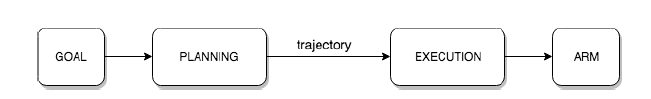
\includegraphics[width=0.75\linewidth]{images/open_loop.png}
    \caption{Open loop architecture}
    \label{pict:open_loop}
\end{figure}

Trajectory is planned, from the current pose to the desired pose, before the manipulator starts its motion. Execution is realized by a trajectory controller from Moveit! framework. The following module takes computed trajectory, which is a sequence of joints angles, converts them into the drivers speed and sends information to the servos of manipulator. 

\subsection{PBVS}

During the period of my internship, another student was working at the time, on the development on a new controller for the manipulator. This work was based on developing an optimization based Cartesian controller for the manipulator (from an input desired pose and the current position of the end effector computing joint velocities to reach the desired pose with constraints on joint position). Combining this work with a pose estimation algorithm developed by another student using also YOLO, a \gls{PBVS} is implemented (\ref{chap:pbvs}). It is using the head camera of the robot, so an EYE-TO-HAND configuration (figure:\ref{pict:eye_in_hand}).
\begin{figure} [!ht]
    \centering
    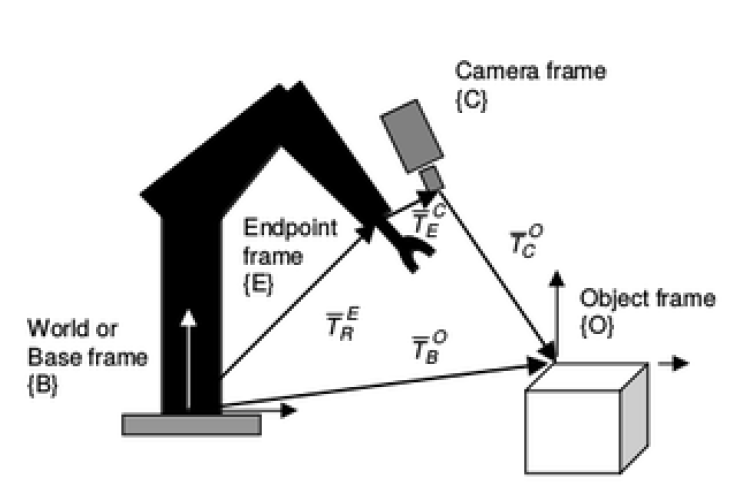
\includegraphics[width=0.95\linewidth]{images/pbvs.png}
    \caption{PBVS architecture developed by another student}
    \label{pict:pbvs_emilia}
\end{figure}

This controller is combining motion of the base and the manipulator. It has been designed as an optimization problem. For now, it applied constraints to avoid joint limits.

\section{Developed solutions}
\label{developed_solution}

\subsection{Approach}
Applying an Image Based Visual Servoing control law to Mbot 7DoF with an EYE-IN-HAND configuration is the subject of this work. This title is describing the working approach. The approach here is to use an \gls{IBVS} (\ref{chap:ibvs}). This control law is applied to a robotic manipulator that has 7 joints and 7\gls{DoF}. The camera is fixed on the end effector that is defined as an EYE-IN-HAND configuration (figure: \ref{pict:eye_in_hand}).
\subsubsection{Constraints}
The constraints for this work are:
\begin{itemize}
    \item Using an IBVS control law with an EYE-IN-HAND configuration
    \item No predefined object, the algorithm as to be as generic as possible
    \item The algorithm has to as close as real time as possible
    \item The working environment is not fixed, it is dynamic, the control law has to adapt to new environment and if the object move during the grasping approach
    \item Having a grasping approach, not only going to a certain pose but also think about grasping
\end{itemize}
\subsubsection{Why using an IBVS}
The two major benefits of using an \gls{IBVS} in a grasping approach are:
\begin{itemize}
    \item Avoiding calibration issues, the precision for grasping is really important, because a small error (cm) can lead to a grasping fail.
    \item Closed loop and able to be use in a dynamic environment
\end{itemize}
In the next subsection, the tools used for this work will be described hardware and software.

\subsection{Hardware and Software}
\label{HardwareSoftware}
To achieved the design and implementation of the previously described approach, we did not start from scratch. We used existing libraries, software and also of course an already very advanced robot  hardware speaking robot, Mbot.
\subsubsection{Software}
\begin{itemize}
    \item 
\gls{ROS} is a middleware (\ref{pict:ros}). It is a computer software that provide services to software applications. It makes easier for software developers to implement communication and input/output, so they can focus on the specific purpose of their application.
\gls{ROS} is a flexible framework helping developers creates software for robots \cite{288}. It provides device drivers, collection of tools and libraries, visualizers, message-passing, package management, and more to simplify the task of creating complex applications across various robotics platforms. ROS is licensed under an open source. Developed controller is implemented in the Robot Operating System environment for the needs of integration the module with the team code base.
\begin{figure} [!ht]
    \centering
    
\includegraphics[width=0.35\linewidth]{images/ros.png}
    \caption{Robot Operating System, since 2007.}
    \label{pict:ros}
\end{figure}
    \item
\gls{ViSP} is a modular C++ library that allows fast development of visual servoing applications \cite{articlevisp}. ViSP is developed and maintained by the Inria Rainbow team located at Inria Rennes. The platform takes the form of a library which is divided in several modules (core, io, gui, vision, …). ViSP software environment features independence with respect to the hardware, simplicity, extendibility, and portability. ViSP also features a large library of elementary tasks with various visual features that can be combined together, an image processing library that allows the tracking of visual cues at video rate, a simulator, an interface with various classical frame grabbers, a virtual 6DoF robot that allows the simulation of visual servoing experiments, etc. The platform is implemented in C++ under Linux.

To use ViSP inside a ROS environment, ViSP ROS package was used. It also have been developed by Inria Rennes. It is an extension of the ViSP library. While ViSP is independent from ROS, in $visp_ros$ we benefit from ROS features.
\begin{figure} [!h]
    \begin{minipage}[b]{0.5\linewidth}
        \begin{center}
            
\includegraphics[width=0.8\linewidth]{images/bandeauViSP.png}
        \end{center}
        \label{pict:visp_logo}
    \end{minipage}
    \begin{minipage}[b]{0.5\linewidth}
      \begin{center}
        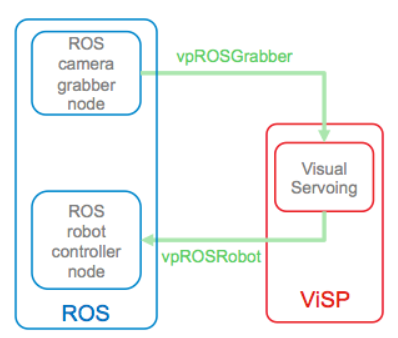
\includegraphics[width=0.6\textwidth]{images/visp_ros.png}
      \end{center}
    \end{minipage}
    \caption  {ViSP, Visual Servoing Platform, developed by Inria Rennes, 2005}
\end{figure}
    \item 
Gazebo is a simulation software that is highly compatible with ROS development. Robot simulation is an essential tool in every roboticist's toolbox. A well-designed simulator makes it possible to rapidly test algorithms, design robots, perform regression testing, and train AI system using realistic scenarios. Gazebo offers the ability to accurately and efficiently simulate populations of robots in complex indoor and outdoor environments.Gazebo is an open source software, improved by the community.
\begin{figure} [!h]
    \begin{minipage}[b]{0.4\linewidth}
        \centering
        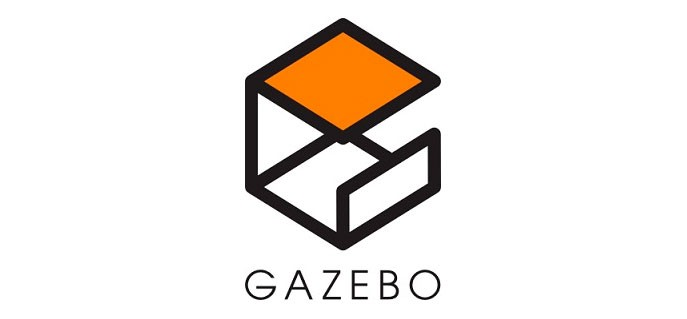
\includegraphics[width=1\textwidth]{images/gazebo.jpg}
    \end{minipage}
    \begin{minipage}[b]{0.6\linewidth}
      \begin{center}
        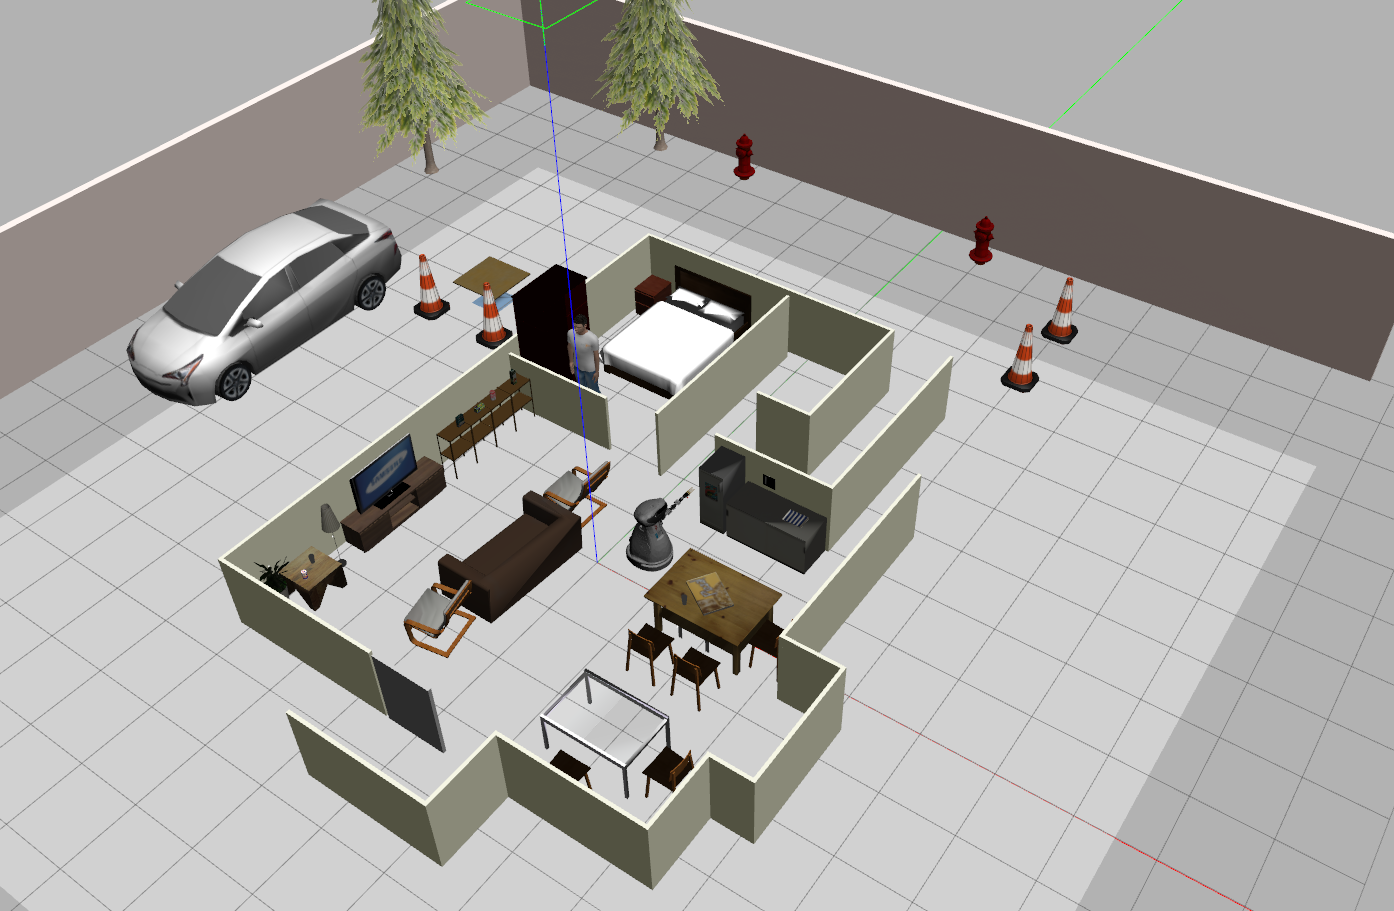
\includegraphics[width=0.8\textwidth]{images/gazebo_isr_testbeld.png}
      \end{center}
    \end{minipage}
    \caption{Gazebo, ROS friendly simulation software(left), ISR testbeld used to test robot tasks in Gazebo (right)}
\end{figure}
    \item 
\gls{URDF} is a package of a number of XML format files, used in \gls{ROS} to describe all elements of the robot. XML files contain specification of sensors, robot models, scenes and more. Each file of XML format has a corresponding in one or more programming language parser. In our project the URDF files contains the most essential information for this work about manipulator (number of joints, links lengths, joints limits, etc.) as well as information about the robotic base. It is also used to construct the robot model in Gazebo for example and in Rviz.
    \item 
\gls{YOLO} is a convolutional neural network used in this work to detect and extract features. It has been described in the the chapter \ref{chapter:Background} in section \ref{Object_detection}.
    \item 
Controlling manipulator servos (sending commands to the joints of the manipulator), to this purpose two possibilities:
    \begin{enumerate}
        \item  An inverse kinematic controller, that take as input a desired velocity vector of the end effector and compute the corresponding joint velocities to achieve the desired velocity for the end effector. This "controller" only controls the manipulator and not the manipulator and the base of the robot combined to be able to reach a larger area when having a grasping approach. The well known problem when using inverse kinematic as described in section \ref{chap:inversekinematics} is singularities and local minima.
        \item An optimization forward kinematic controller, developed during the time of my internship to use with his work on \gls{PBVS}. This "controller" controls the manipulator and the base at the same time. It takes as input a pose in world frame and output the joint velocities, more information on the section \ref{Previous_architecture}. Since it is an early development many problems appeared using this controller, like when doing the optimization not using the last joint or not taking as input velocities. One of my work was to convert this controller to be able to end effector velocities as input.
    \end{enumerate}

\end{itemize}

\subsubsection{Hardware}
\begin{itemize}
    \item Manipulator description
The manipulator used by the robot is a Cyton Gamma 1500 (figure: ) produced by Robai company. It is a 7DoF manipulator with a 3D printed end effector. Joints of the manipulator are made of two types of DYNAMIXEL smart actuators: MX-28 and MX-64 (figure:).
As it’s written in the product documentation, humanoid robot arms with many degrees of freedom, can reach around obstacles and through gaps, reconfigure for strength, and manipulate objects with dexterous fluid motion. This manipulator has kinematic redundancy, that enables placement of a hand or tool at a position and orientation in an unlimited number of ways. Presented manipulator model is no longer commercially available.
\begin{figure} [!ht]
    \begin{minipage}[b]{0.5\linewidth}
        \centering
        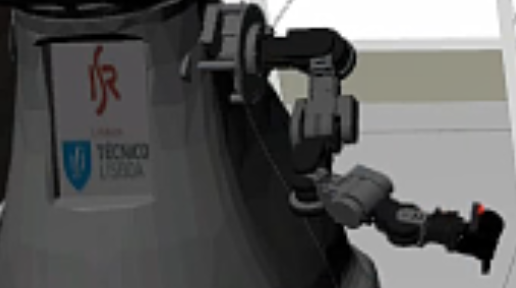
\includegraphics[width=0.8\textwidth]{images/manipulator_sim.png}
    \end{minipage}
    \begin{minipage}[b]{0.5\linewidth}
      \begin{center}
        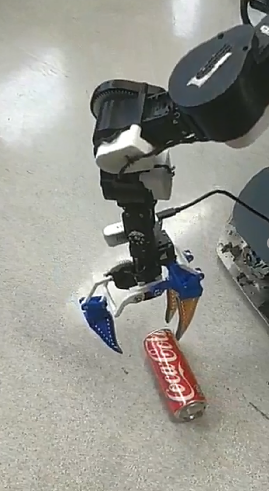
\includegraphics[width=0.35\textwidth]{images/real_robot_grasping_floor.png}
      \end{center}
    \end{minipage}
    \caption{Manipulator in simulation with Gazebo and defined by an \gls{URDF} file(left), Real manipulator fixed on Mbot (right)}
\end{figure}


\newpage
    \item 
The Intel® RealSense™ Depth Camera D435 uses stereo vision to calculate depth. It is USB-powered and consist of a pair of depth sensors, an RGB sensor, and an infrared projector. It is a close ranged depth camera that can read depth from about 0.17m to 0.8m. It is also really compact and light that makes this camera perfect for being fixed on the end effector.
\begin{figure} [!ht]
    \centering
    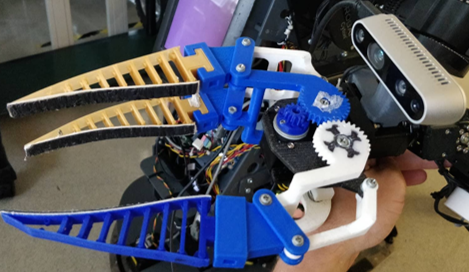
\includegraphics[width=0.5\linewidth]{images/camera_and_gripper_real.png}
    \caption{Camera and effector on Mbot}
    \label{pict:camera_gripper}
\end{figure}
\end{itemize}

In the next subsections we will present the developed solutions. The work will be divided in two part: a first solution and a final solution. When I start my internship, the robot was not equipped with the gripper camera fixed on the manipulator effector and before implementing your algorithm, it is usual to first test it inside simulation. So, he first implementation has been developed in simulation and the final solution has been implemented in simulation and inside the real robot. The main difference between these solutions is the way its initialized and the way the features are detected and extracted.

\subsection{1st solution: Blob tracking}
  
The first solution is based on a simple feature detection and tracking method called blob detection and tracking. Blob detection methods aimed at detecting regions in an image that differ in properties such as color, brightness for example compared to surrounding regions.A blob is a region of an image in which properties defined are constant or approximately constant. In simulation this blob are black points on a juice box.
The first step of this control scheme is the initialization, the user as to click with the mouse inside the display on the 4 dots. From these blobs, the \gls{COG} is computed : 4 image points with (x,y) coordinates.
From this image point, 4 features are computed. The depth is computed from the surface of the blob using image moment and a scale factor.
Desired features have been create previously depending which position of the gripper you want. Then the error is computed (to see how the error, the interaction matrix and finally the control is computed refer to section \ref{chap:ibvs}.
\begin{figure} [!h]
    \centering
    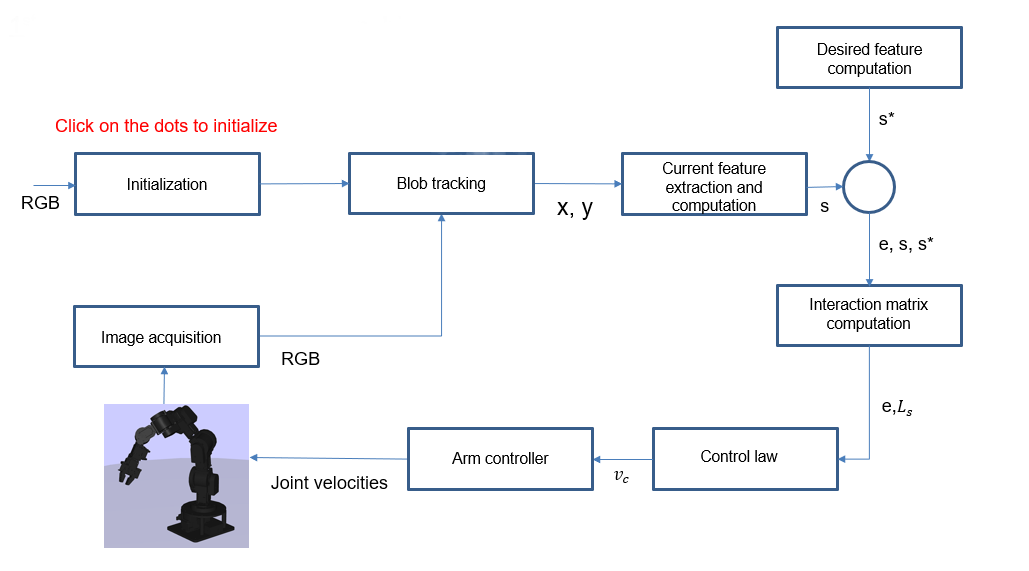
\includegraphics[width=0.95\linewidth]{images/control_scheme_1.png}
    \caption{First solution control scheme}
    \label{pict:control_scheme_1}
\end{figure}

The interaction matrix computed from 4 points is:
\[
L_s
=
\begin{bmatrix}
    - \frac{1}{Z_1} & 0 & \frac{x_1}{Z_1} & x_1 y_1 & -(1+x_1^2) & y_1 \\
    0 & - \frac{1}{Z_1} & \frac{y_1}{Z_1} & 1+y_1^2 & - x_1 y_1 & x_1  \\
    - \frac{1}{Z_2} & 0 & \frac{x_2}{Z_2} & x_2 y_2 & -(1+x_2^2) & y_2 \\
    0 & - \frac{1}{Z_2} & \frac{y_2}{Z_2} & 1+y_2^2 & - x_2 y_2 & x_2  \\
    - \frac{1}{Z_3} & 0 & \frac{x_3}{Z_3} & x_3 y_3 & -(1+x_3^2) & y_3 \\
    0 & - \frac{1}{Z_3} & \frac{y_3}{Z_3} & 1+y_3^2 & - x_3 y_3 & x_3  \\
    - \frac{1}{Z_4} & 0 & \frac{x_4}{Z_4} & x_4 y_4 & -(1+x_4^2) & y_4 \\
    0 & - \frac{1}{Z_4} & \frac{y_4}{Z_4} & 1+y_4^2 & - x_4 y_4 & x_4  
\end{bmatrix}
=
\begin{bmatrix}
    L_{x1} \\
    L_{x2} \\
    L_{x3} \\
    L_{x4} 
\end{bmatrix}
\]
To approximate the pseudo inverse matrix of the interaction matrix, we use the minimization approach :
\[
\Hat{L_s^+} = \frac{1}{2}(L_{s^*}^+ + L_s^+)
\]
with $L_{s^*}$, the interaction matrix similar to $L_s$ above but computed with the desired features.
From this interaction matrix, the control law is compute:
\begin{equation}
\begin{bmatrix}
    v_x \\
    v_y \\
    v_z \\
    w_x \\
    w_y \\
    w_z
\end{bmatrix}
= - \lambda L_{s}^+ 
\begin{bmatrix}
    e_{x_1} \\
    e_{y_1} \\
    e_{x_2} \\
    e_{y_2} \\
    e_{x_3} \\
    e_{y_3} \\
    e_{x_4} \\
    e_{y_4} 
\end{bmatrix}
\end{equation}
The gain $\lambda$ is computed using an adaptive gain. It is a varying gain as:
\begin{equation}
    \lambda(||e||)
    = 
    (\lambda_0 - \lambda_\infty)
    e^{-\frac{\lambda_{0}^{'}}{\lambda_0 - \lambda_\infty}}
    + \lambda_\infty
\end{equation}
with $\lambda_0$, the gain for very small values of $||e||$, $\lambda_\infty$, the gain for very high values of $||e||$ and $\lambda_{0}^{'}$, the slope of $\lambda$ at $||e|| = 0$.
The computed velocities are Cartesian camera velocities but since the camera is fixed on the end effector, we assume that it is the end effector Cartesian  velocities. 
This vector is send to the manipulator controller that compute with inverse kinematic or optimization forward kinematic the joint velocities of the manipulator. Acquiring a new image and applying the same steps close the loop.

\begin{figure} [!ht]
    \begin{center}
        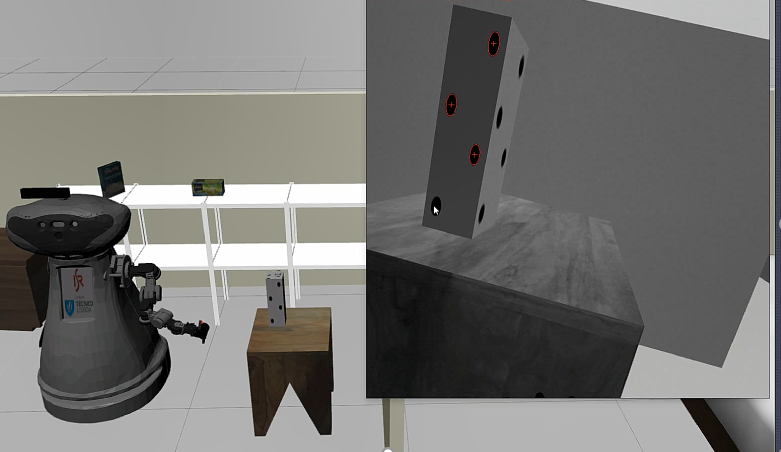
\includegraphics[width=0.8\linewidth]{images/blob_tracking.png}
    \end{center}
    \begin{center}
        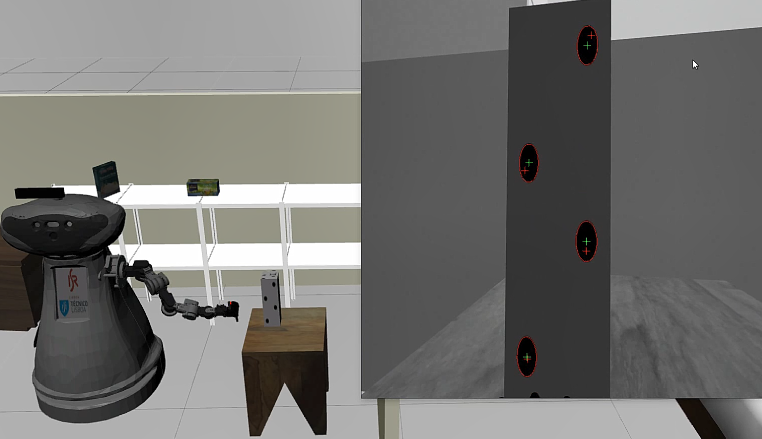
\includegraphics[width=0.8\textwidth]{images/reach_blob_tracking.png}
    \end{center}
    \caption  {Blob tracking IBVS Initialization (top), Blob tracking IBVS desired end effector pose reached (bottom), in gazebo}
     \label{pict:blob_tracking_reach}
\end{figure}

On figure \ref{pict:blob_tracking_reach}, the top picture shows the initialization where the user as to click on the blob (black points) to initialize the algorithm. In this picture the red cross represent the current features. In the bottom picture, the manipulator reached the desired pose for the end effector, the current features (green cross) are matching the desired features (red cross). 

\subsubsection{Result for the first implementation}

The manipulator reach the correct pose requested by the user (as it has been hardcoded by the position of the desired features in the image). With this method the 6DoF of the camera are controlled. Using the inverse kinematic controller, it is possible to compute the 7 joint velocities of the manipulator to apply the desired end effector velocity. This first implementation has been successfully implemented using the inverse kinematic Cartesian controller and the optimization forward kinematic controller (section:\ref{HardwareSoftware}). 

It is only working in simulation, because having blob like this on a juice box, is not possible in real environment and the computation of the depth from the size of this blob would be really not precise (due to different lighting, different size of dots, ...). And for the main reason that at that time of my internship no camera were available fixed on the gripper, only in simulation.\\

To resume this first implementation :
\begin{itemize}
    \item Progress
    \begin{enumerate}
        \item IBVS visual servoing implemented in gazebo with both manipulator controllers.
        \item Using blob tracking and 4 points, 6DoF are controlled
        \item Depth computation from the surface of the blob
    \end{enumerate}
    \item Drawbacks
    \begin{enumerate}
        \item Blob tracking is not generic for different object types and not robust
        \item Depth computation not robust
        \item No real implementation
    \end{enumerate}
\end{itemize}

\begin{figure}[!ht]
     \centering
     \subfloat{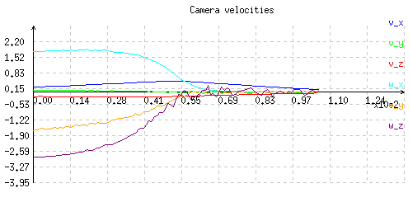
\includegraphics[width=0.495\linewidth]{images/courbe_4pts_blob_tracking_1.png}}\label{<figure_simulation_1>]}
     \subfloat{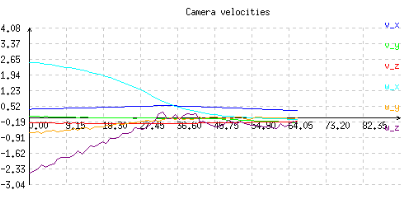
\includegraphics[width=0.495\linewidth]{images/courbe_4pts_blob_tracking_2.png}}\label{<figure_simulation_2>]}
     \caption{Camera velocities evolution during time, blob tracking method in simulation from different starting arm position}
     \label{pict:plot_simulation_2}
\end{figure}
In figure \ref{pict:plot_simulation_2}, the exponential decrease is visible for the 6 velocities, it converges asymptotically and oscillations are very small (except for the z rotation, but this is due to the arm controller), the trajectory is smooth.

\subsection{Final solution: YOLO center bounding box}

Looking at the first solution implemented and described in the previous section, the controller is not generic and not robust. Indeed, there are no black dots like in simulation in a real environment with real object. Also, when the manipulator is moving even in simulation or if the gripper goes in front of one dot, features are lost and the controller get stuck, so  definitely not robust. 

It was time to find a new solution, more generic for multiple objects, more robust to manipulator motions and of course that suit more for a real environment implementation . The idea came to use a neural network already running inside the robot called YOLO (see section: \ref{Object_detection}). YOLO is trained with a set of objects, for example the objects that could be grasp inside the home environment. After this step, the algorithm is able to process as an object detection algorithm, giving the position of the object in the image (via a bounding box) and to classify the object (via class name, name of the object). 

It is more robust to object occlusion or losing the object when moving than blob tracking. The main reason is that even if the object is only partially in the image, YOLO is still able to detect it. Also, It can be train with multiple real objects so It really suit an implementation in a real environment and of course from the fact that it can be trained with multiple objects makes it more generic. From the first solution implementation, it is improved our control law. 

\begin{figure} [!h]
    \centering
    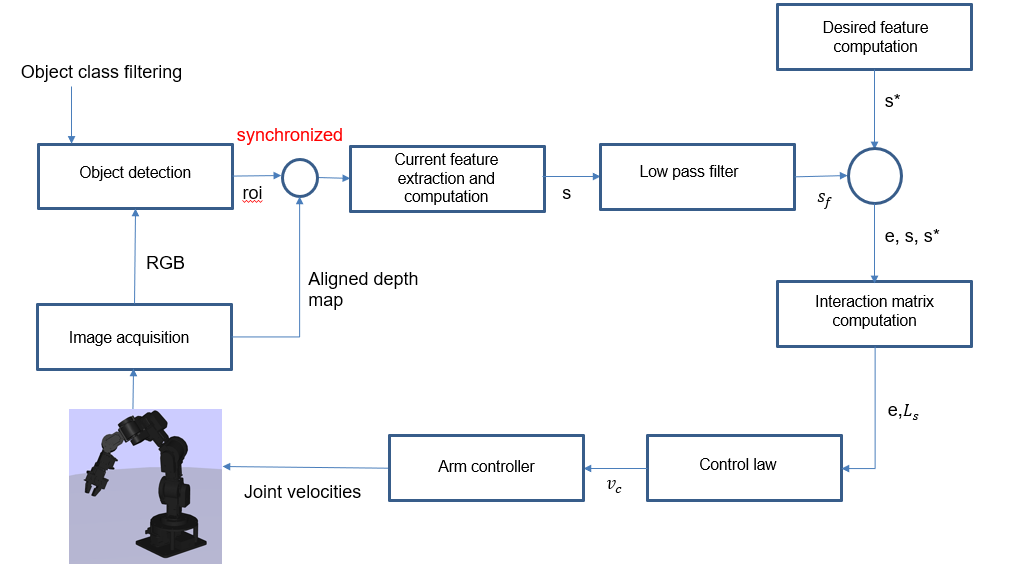
\includegraphics[width=1\linewidth]{images/final_control_scheme.png}
    \caption{Final solution control scheme}
    \label{pict:control_scheme_final}
\end{figure}

From YOLO bounding box, the controller algorithm extract the \gls{COG}, one point with (x,y) coordinates. Synchronized with the previous, the aligned depth map is received and convert to the proper unit. The next step is to compute the current feature from the point coordinates and the depth.
Using the COG of the bounding box gives only one 2D point. If we only use this point like one from the previous solution, the controller would only control 2DoF because the interaction matrix will be of rank 2. To be able to at least control all DoF in translation, it is possible to create a third parameter from a 2D point $z = log( Z/Z^*)$, that defines the current depth ($Z$) relatives to the desired depth ($Z^*$) and so $s = (x, y, z)$. \\

The next step is to filter the feature position. The algorithm use a low pass filter to attenuate the variation of the position of the \gls{COG}. Indeed, the motion of the arm and even the own vibrations of the manipulator makes the position of the bounding box really unstable, applying a low pass filter smooth these variations and makes easier to reach match the current feature and the desired one.
The low pass filter equations used are:
\[
    x_{center+1} = x_{center} + \lambda*(x - x_{center}) 
\]
\[
    y_{center + 1} = y_{center} + \lambda*(y - y_{center})
\]
The current feature is also created from a desired point in the image $s^*=(x, y, Z)$. The next step is to compute the error vector and the interaction matrix. The interaction matrix will be different from the one of the first implementation because only one point will be used and the feature used has three parameters (x, y, z) and not only two (x,y):
\[ 
Ls
=
\begin{bmatrix}
    - \frac{1}{Z_1} & 0 & \frac{x_1}{Z_1} & x_1 y_1 & -(1+x_1^2) & y_1 \\
    0 & - \frac{1}{Z_1} & \frac{y_1}{Z_1} & 1+y_1^2 & - x_1 y_1 & x_1  \\
    0 & 0 &  - \frac{1}{Z_1} & -y_1 & x_1 & 0
\end{bmatrix}
\]
The steps to compute the interaction matrix are exactly the same than the one presented in section \ref{chap:ibvs} but with using the extra parameters per feature $ z = log(Z/Z^*)$
With only one point and with this interaction matrix, it is possible to compute the 3 linear velocities (velocities translational motions only, not rotational). This method is refereed as 2-1/2D hybrid visual servoing in section \ref{hybrid}. This algorithm will only control the translational motion of the camera. A 3D pose estimation algorithm would have to be add in future work to compute the rotational motion.
To estimate the interaction, the same from previous solution minimization method is used:

\[
\Hat{L_s^+} = \frac{1}{2}(L_{s^*}^+ + L_s^+)
\]\\

The control law computed from this interaction matrix is:
\begin{equation}
\begin{bmatrix}
    v_x \\
    v_y \\
    v_z 
\end{bmatrix}
= - \lambda L_{s}^+ 
\begin{bmatrix}
    e_{x_1} \\
    e_{y_1} \\
    e_{z_1}
\end{bmatrix}
\end{equation} \\
The same adaptive gain is used for $\lambda$, refer to previous solution for more details. 
The last step is to send the velocities to the end effector. 
This final solution was implemented in simulation first and then inside the real robot.\\

In figure \ref{pict:yolo_simulation_real}, the green cross represents the current feature $s$ and the red cross represent the desired feature $s^*$. 

\begin{figure}[!ht]
     \centering
     \subfloat{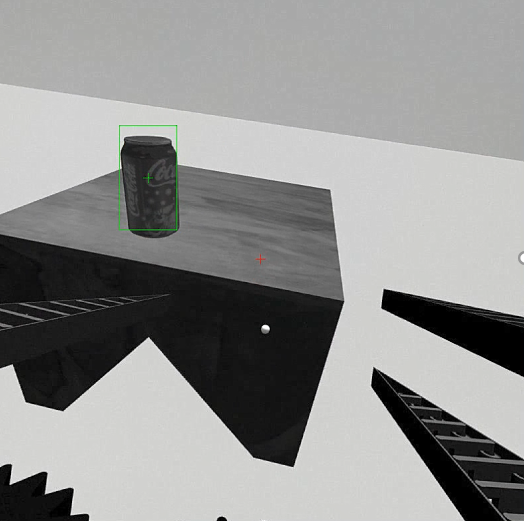
\includegraphics[width=0.43\textwidth]{images/yolo_simulation.png}}\label{<figure_simulation>]}
     \subfloat{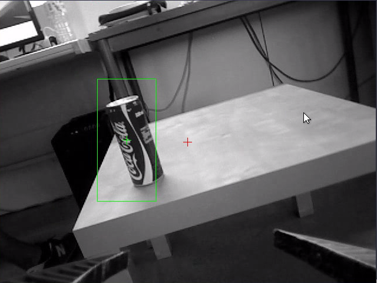
\includegraphics[width=0.563\textwidth]{images/yolo_real.png}}\label{<figure_real>]}
     \caption{YOLO center bounding box method in simulation (left), YOLO center bounding box method in real robot (right)}
     \label{pict:yolo_simulation_real}
\end{figure}

On the left picture of figure \ref{pict:yolo_simulation_real}, the YOLO center bounding box method is shown inside gazebo. YOLO can also be trained with real objects and work in simulation with the same simulated objects.

On the right picture of figure \ref{pict:yolo_simulation_real}, the final solution is running inside the real robot using the Intel realsense D435 camera.

\subsubsection{Results for the final implementation}

The manipulator reach the correct pose requested by the user as it has been hardcoded by the position of the desired features in the image, here the center of the gripper. With this method only 3DoF of the camera are controlled. Using the inverse kinematic controller, it is possible to compute the 7 joint velocities of the manipulator to apply the desired end effector velocity. This final implementation has been successfully implemented  in gazebo simulation and inside the real robot using the inverse kinematic Cartesian controller only (section:\ref{HardwareSoftware}). For unknown reasons at the moment, this algorithm is not working with the optimization forward kinematic controller but it is an implementation error not a theoretical. \\

In the figure \ref{pict:yolo_simulation_plot}, the exponential decrease is visible for the 3 velocities, it converges  and oscillations are very small (except for the z rotation, but this is due to the arm controller), the trajectory is smooth. \\

In simulation, the "working" conditions are perfect (arm calibrations, camera calibrations, lighting, objects always similar). It is not a surprise to have such results.
\newpage
\begin{figure} [!h]
    \centering
    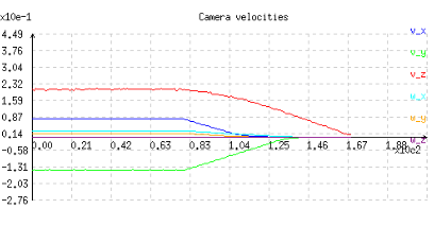
\includegraphics[width=0.6\linewidth]{images/yolo_plot_simulation.png}
    \caption{Camera velocities evolution during time, using YOLO center bounding box method}
    \label{pict:yolo_simulation_plot}
\end{figure}

The difference between an implementation in simulation and in a real environment is illustrated by the difference between \ref{pict:yolo_simulation_plot} and \ref{pict:yolo_real_plot}. It is obvious that first the trajectory is less smooth and the oscillations are more important in a real environment. 

Figure \ref{pict:yolo_real_plot} is showing the evolution of the camera velocities during time. In the top graphic of figure \ref{pict:yolo_real_plot}, it starts to converge but finally diverge with strong oscillations. \\

It can be due to contradictory velocities send to the arm controller created by oscillations of the arm due to the controller having difficulties to find a solution to the inverse kinematic problem. In chain oscillations of the manipulator create an image and feature that change of position more frequently and with more offset that in chain compute wrong velocities to the arm controller. 

The inverse kinematic Cartesian controller not finding a solution to reach the desired end effector velocities can be due to falling into a singularity problem. There are various type of cause to singularities but with a manipulator with 7DoF and 7 joints it is mostly due to the fact that there are an infinite number of solutions and without adding constraints to the problem, the arm controller is not able to choose one. Multiplying the features is a way to avoid singularities.

It can also be due to the fact that the object is not reachable in the actual position of the arm, the arm controller keeping trying to reach the desired position create oscillation that as the effect described before.

Another issue, that has been encountered but that cannot be illustrated by this graphic because it would not be visible is falling into local minima. It is due to the approximation of the interaction matrix that might be not full rank and the system get trap in a local minimum. In this graphic that would mean that all velocities values have converged to 0 but the pose of the end effector is not the one desired, $e \neq 0$ but $ \hat e = 0$. \\

When not falling into singularities or local minima, an exponential asymptotic convergence can be observed like in the bottom graphic of the figure \ref{pict:yolo_real_plot}.
\newpage
\begin{figure}[!ht]
     \centering
     \subfloat{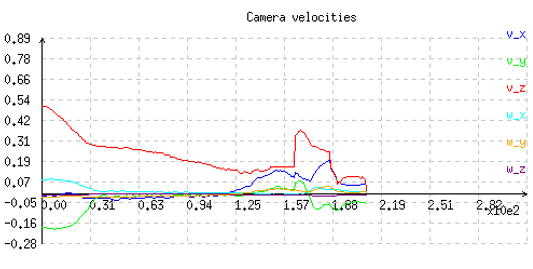
\includegraphics[width=0.7\textwidth]{images/courbe_yolo_1.png}}\label{<figure_simulation>]}
     \subfloat{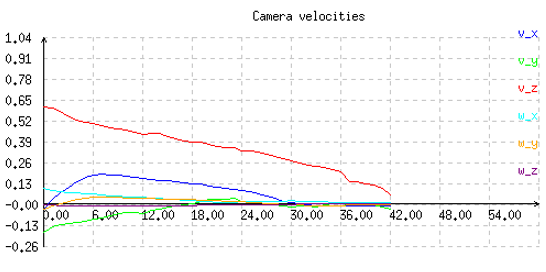
\includegraphics[width=0.7\textwidth]{images/courbe_yolo_2.png}}\label{<figure_real>]}
     \caption{Evolution of the camera velocities during time, using YOLO center bounding box method in real robot}
     \label{pict:yolo_real_plot}
\end{figure}

To resume this final implementation :
\begin{itemize}
    \item Progress
    \begin{enumerate}
        \item 
IBVS visual servoing implemented in gazebo and inside real robot with inverse kinematic Cartesian controller.
        \item 
Using YOLO center point box, 1 feature, 3DoF are controlled, only translational motions but very generic algorithm
        \item 
Depth computation from Intel camera D435, aligned to RGB image and synchronized with YOLO bounding box up to 16 cm (object already inside the gripper).
        \item
Robust to dynamic environment (moving object for example), to arm motions and to partial obstructions of the object (because partially in the image or because gripper finger in front)
        \item 
Algorithm real time
    \end{enumerate}
    \item Drawbacks
    \begin{enumerate}
        \item The object has to stay in sight. 
        \item Singularities and local minima from the compute of the control law and from the inverse kinematic Cartesian controller.
        \item No rotational motions control 
    \end{enumerate}
\end{itemize}




